%************************************************
\chapter[Multiple Interactions Networks]{Multiple interactions networks: towards more realistic
descriptions of the web of life}\label{ch:review}
%************************************************

%\tikz[remember picture,overlay] \node[opacity=0.3,inner sep=0pt] at (current page.center){
\includegraphics[width=\paperwidth,height=\paperheight]{./Figures/cover/Goya_Dog.jpg}};
\tikz[remember picture,overlay] \node[opacity=0.3,inner sep=0pt] at ([yshift=3cm,xshift=2cm]current page.center){
\includegraphics[width=\paperwidth,height=\paperheight]{./Figures/cover/Goya_Dog.jpg}};
\clearpage

\section*{Abstract}
Ecological communities are defined by species interacting dynamically in a given location at a given time, and can be conveniently represented as networks of interactions. Pairwise interactions can be ascribed to one of five main types, depending on their outcome for the species involved: amensalism, antagonism (including predation, parasitism and
disease), commensalism, competition or mutualism. While most studies have dealt so far with networks involving one single type of interaction at a time, often focusing on a specific clade and/or guild, recent studies are being developed that consider networks with more than one interaction type and across several levels of biological organisation. We review these developments and suggest that three main frameworks are in use to investigate the properties of multiple interactions networks: ‘expanded food-webs’, ‘multilayer networks’ and ‘equal footing networks’. They differ on how interactions are classified and implemented in mathematical models, and on whether the effect of different interaction types is expressed in the same units. We analyse the mathematical and ecological assumptions of these three approaches, and identify some of the questions that can be addressed with each one of them. Since the overwhelming majority of studies on multiple interactions are theoretical and use artificially generated data, we also provide recommendations for the incorporation of field data in such studies.

\section{Community ecology and network theory}
Ecological communities should be defined not only by lists of co-occurring species, but also by the myriad of interactions taking place among them. A convenient way to include information about both species composition and their interactions is to represent communities as networks in which species are nodes connected by links representing biotic interactions. Network analyses can provide insights into community local stability \citep{Allesina2012} and robustness to extinctions \citep{Riede2011a}, the degree of specialization of individual species or guilds \citep{Dorado2011}, the impact of invasive species or climate change on established communities \citep{Lopezaraiza-Mikel2007} and, more generally, on any question in which pairwise interactions relate to community patterns and processes.

Networks can accommodate different types of data, depending on the nature of the links between species (e.g., qualitative, quantitative, static, dynamic), the temporal and spatial resolution of the community, the level of aggregation of the nodes (e.g., individuals, species, trophic guilds), or the specific objectives of the study. A common simplification is to study networks of a single interaction type, e.g., trophic \citep{McCann2011} or mutualistic \citep{Bascompte2013}, assuming (often implicitly) that the effect of other interactions on community dynamics is negligible compared to the ones analysed. Such an assumption is usually unavoidable given the lack of comparable data on different interaction types, but it is becoming increasingly clear that the effects of interactions not accounted for in analyses of single-interaction networks (including indirect ones; but see \citealt{Cazelles2016}) might be significant for species persistence \citep{Soliveres2015a, Kefi2016a} and community structure \citep{Sander2015, Golubski2016}. Furthermore, analyses of interaction networks of a single type often yield differential results regarding the factors that drive their stability. For example, among the factors reported to stabilize food webs are high modularity and low connectance \citep{Thebault2010}, correlation in pairwise interaction strengths \citep{Tang2014}, trophic coherence \citep{Johnson2014}, a preponderance of weak \citep{McCann1998} and asymmetrical interactions \citep{Bascompte2006}, degree distributions broader than those of random graphs \citep{Allesina2015}, or the appearance of generalist consumers coupling resources with different interaction strengths \citep{Rip2010}. On the other hand, mutualistic networks are thought to be more stable when highly nested and connected \citep{Thebault2010, Lever2014}, when there are demographic responses to interactions \citep{Lee2015}, or when mutualistic interactions are relatively strong \citep{Rohr2014}. The persistence and resilience of communities defined with multiple interaction types, however, will additionally likely be influenced at least by (1) the proportion of the different interaction types, (2) the relative strength of pairwise interactions both within and among interaction types, and (3) the structural properties of each sub-network and the overall aggregated network.

The study of single-interaction networks in ecology has progressed enormously in the last decades, both theoretically and empirically. In parallel, the analysis of multiple interactions networks has also advanced in other fields of study \citep{Boccaletti2014}. This novel paradigm has only recently started to be applied to ecological studies, with several examples of new conceptual developments being forged together with applications of old concepts to new problems (Table \ref{tab:table1.1}). Despite the relatively small number of studies using multiple interactions networks in ecology, the research objectives and methodologies that have been addressed are extremely diverse, and a synthesis of recent developments is timely. Here, we identify three main approaches for the design and analysis of ecological multiple interactions networks. These approaches have been used in theoretical and empirical studies without an explicit recognition of their conceptual underpinnings. We define them explicitly, examine their underlying ecological assumptions, the type of questions best addressed with each approach, and provide recommendations for the integration of empirical data.

\section{Multiple interactions networks in ecology}
Probably, the first study of ecological networks explicitly considering different interaction types was the classic study by \cite{May1972}, in which he assembled interaction matrices with random coefficients from a Gaussian distribution  $N{\sim}\left(0,\sigma \right)$  , thereby allowing for negative and positive pairwise interactions to be considered. May's results showed that in theoretical communities assembled randomly, complexity (measured as connectance and species richness) was inversely related to the local stability of the system. But natural communities are highly complex, diverse and, nonetheless, seem to persist. After that seminal study, there has been a flurry of studies trying to uncover the processes and structural patterns that confer stability to empirical communities (e.g. \citealt{Saint-Beat2015}). However, comparable data on different interaction types is extremely difficult to acquire, and the focus for most of the second half of the 20th century has been on how competitive and antagonistic interactions drive population and community patterns (e.g. \citealt{Connell1961, Paine1966}). As predator-prey interactions are easiest to observe and document in the field, the analysis of empirical networks relied almost entirely on food webs for a few decades. Pioneering works by \cite{Jordano1987}, or \cite{Fonseca1996}, amongst others, paved the way for the study of mutualistic networks, but the first studies considering more than one interaction type in the same network only appeared in the last decade (Table \ref{tab:table1.1}).

Developing a theoretical framework for multiple interactions networks involves the integration of a variety of interaction types and effects, direct and indirect, taking place at different temporal and spatial scales. In this review, we propose two main criteria for classifying such frameworks. The first is the classification system applied to interactions \citep{Abrams1987}. Interactions can be defined based on the effect they produce on each member or, alternatively, on the mechanism by which the interaction is produced. Regarding effects, each interactor can be affected positively, negatively, or not affected at all by a pairwise interaction, regardless of the actual mechanisms by which the effect occurs. For example, a (-,-) interaction, defined as competition, could actually be realized through mechanisms as different as territorial, chemical or consumptive competition \citep{Schoener1983}. By defining all interactions with respect to the effect on each member (0,-,+), every effect-based classification is complete, in the sense that no interaction, however idiosyncratic, is left unclassified. Regarding mechanisms, interactions are defined according to the mechanism by which they take place, regardless of the effect on the interacting species. Thus, consumptive competition would be defined as an interaction in which each member is affected by consumption of a common limited set of resources, territorial competition would represent limitations on the available space for each interactor, and so on. A virtually unlimited number of interaction categories can be theoretically defined under this scheme, depending on the questions addressed.

The second criterion distinguishes network analyses based on whether the strengths of different interaction types have common units (i.e., their effects are comparable, acting upon the same population property) or not. This criterion only applies to classification schemes based on effects as, by definition, strengths of interactions acting explicitly through different mechanisms have different units, and are thus not amenable to being homogenized. For example, chemical competition between two plant species may be reflected on the mortality rates of the interacting populations, while a mutualistic interaction between a plant species and a seed disperser bird may affect the dispersal rate of the plant and the population growth rate of the bird. In an effect-based classification with the same units for every interaction, on the contrary, these and every other interaction could be taken to affect a single property (e.g. long-term population size), and hence would be comparable. Based on the two criteria proposed here, we distinguish three conceptual frameworks, already found in the literature, to construct and analyse multiple interactions networks: expanded food webs, multilayer networks, and equal footing networks (Fig. \ref{fig:fig2.1}).

%\afterpage{
%\clearpage% Flush earlier floats (otherwise order might not be correct)
%\thispagestyle{empty}% empty page style (?)
\begin{landscape}% Landscape page
\begin{footnotesize}
%\begin{longtable}{p{1.5cm}p{1.5cm}p{2cm}p{2cm}p{1.5cm}p{2cm}p{4cm}}
\begin{longtable}{p{1.5cm}p{1.5cm}p{2cm}p{2cm}p{2cm}p{2cm}p{4cm}}
\caption[Studies of multiple interactions networks]{\color{Gray}Studies considering networks of more than one interaction type. Analyses of small network modules ({\textless}5 species) are not included\label{tab:table1.1}}\\\hline
Study & Framework &  Type of classification & Interaction types studied & Interaction strength  &  Type of data & Main findings\\\hline
\endfirsthead
\hline
Study & Framework &  Type of classification & Interaction types studied & Interaction strength  &  Type of data & Main findings\\\hline
\endhead

\citealt{Arditi2005} & %Arditi et al. 2005  &
Expanded food web &
Mechanism-based &
+ and -- modifications to trophic interactions &
Model coefficient &
Synthetic &
Communities with positive non-trophic interactions tend to incorporate almost all available nutrients\\%\hline
\citealt{Lafferty2006} &%Lafferty et al. 2006 &
Expanded food web &
Mechanism-based &
Predator-prey and several parasitic interactions &
Binary &
Empirical data from four food webs containing parasites &
Links involving parasites are a majority in food webs, and their inclusion modifies structural metrics\\%\hline
\citealt{Goudard2008} & %Goudard and loreau 2008 &
Expanded food web &
Mechanism-based &
+ and -- modifications to trophic interactions &
Model coefficient &
Synthetic &
Interaction webs that include trophic and non-trophic interactions are expected to have a lower local richness, biomass, and production than food webs that include only trophic interactions\\%\hline
\citealt{Lafferty2008} & %Lafferty et al. 2008 &
Expanded food web &
Mechanism-based &
Predator-prey and several parasitic interactions &
N.A. &
N.A. &
Lines of research to integrate parasitic interactions into food webs\\%\hline
\citealt{Kefi2012} & %K\'efi et al. 2012 &
Expanded food web &
Mechanism-based &
N.A. &
N.A. &
N.A. &
Conceptual framework for including non-trophic interactions in food web studies.\\%\hline
\citealt{Donadi2013} & %Donadi et al. 2013 &
Expanded food web &
Mechanism-based &
Effects of allogenic ecosystem engineers &
Measurements of clorophyll content in sediment &
Empirical experiment &
Facilitation of ecosystem-engineering cockles in benthic primary producers on intertidal flats\\%\hline
\citealt{Majdi2014} & %Majdi et al. 2014 &
Expanded food web &
Mechanism-based &
Effects of predators (flatworms) on litter decomposition and community assembly &
Carbon content in leafs, biomass of different guilds, sediment content  &
Empirical experiment &
Flatworms have significant effects on the variables measured, overriding direct trophic effects\\%\hline
\citealt{Sanders2014} & %Sanders et al. 2014 &
Expanded food web &
Mechanism-based &
Different effects of ecosystem engineers &
N.A. &
N.A. &
Integration of ecosystem engineering effects into food web analyses\\%\hline
\citealt{Bachelot2015} & %Bachelot et al. 2015 &
Expanded food web &
Mechanism-based &
Antagonistic, competitive, mutualistic &
Model coefficient &
Synthetic &
Under certain conditions, a balance of different interaction types increases persistence of plant species interacting with mycorrhizal fungi and predators\\%\hline
\citealt{Kefi2016a} & %K\'efi et al. 2016 &
Multilayer network analysed as an expanded food web model &
Mechanism-based &
Trophic and several non-trophic types &
Frequency of interaction between species of the modelled guilds &
Field surveys for species identification and expert knowledge for interaction assignment &
Species are organized in clusters of interaction patterns, and this patterning enhances community persistence and robustness\\%\hline
\citealt{Fontaine2011} & %Fontaine et al. 2011 &
Multilayer network &
N.A. &
N.A. &
N.A. &
N.A. &
Conceptual study on the consequences and challenges of merging two sub-networks\\%\hline
\citealt{Pocock2012} & %Pocock et al. 2012 &
Multilayer network &
Mechanism-based &
Trophic, mutualistic of several types and parasitic &
Interaction frequency &
Field surveys and published studies for assigning interactions &
Different sub-networks varied in their robustness to random extinctions of plants\\%\hline
\citealt{Evans2013a} & %Evans et al. 2013 &
Multilayer network &
Mechanism-based &
Trophic, mutualistic of several types and parasitic &
Interaction frequency &
Field surveys and published studies for assigning interactions &
Habitats of an agro-ecosystem contribute differentially to species and interaction diversity\\%\hline
\citealt{Kefi2015} & %K\'efi et al. 2015 &
Multilayer network &
Mechanism-based &
Trophic, positive non-trophic and negative non-trophic &
Binary &
Field surveys for species identification and expert knowledge for interaction assignment &
Non-trophic interactions are more than twice as abundant than trophic ones, and show non-random structure\\%\hline
\citealt{Sander2015} & %Sander et al. 2015 &
Multilayer network &
Effect-based (tatoosh island and doñana networks), Mechanism-based (norwood network, which differentiates herbivory and parasitism) &
Three networks with different types &
Binary &
Different for each dataset &
Accounting for different interaction types can improve groupings of species in interaction networks\\%\hline
\citealt{Dattilo2016} & %D\'attilo et al. 2016 &
Multilayer network &
Mechanism-based &
Different types of mutualistic interactions &
Binary &
Field surveys for qualitative interactions &
Multiple types of mutualism do not increase community robustness, but a few species contribute disproportionally to network structure.\\%\hline
\citealt{Gracia-Lazaro2018} & %Gracia-l\'azaro et al. 2017 &
Multilayer network &
Effect-based &
Competition (intra-layer) and mutualism (inter-layer) &
Model coefficients &
Adjacency matrices from several plant-pollinator empirical networks &
The intensity of mutualism and competition jointly influences species persistence\\%\hline
\citealt{Pilosof2017} & %Pilosof et al. 2017 &
Multilayer network &
N.A. &
N.A. &
N.A. &
N.A. &
Framework and examples for applying multilayer networks to ecological questions\\%\hline
\citealt{Bastolla2009} & %Bastolla et al. 2009 &
Equal footing network &
Effect-based &
Competition and mutualism &
Model coefficient &
Synthetic &
Nested structure of mutualist networks increases community size\\%\hline
\citealt{Melian2009} & %M\'elian et al. 2009 &
Multilayer network flattened to an equal footing model &
Effect-based &
Antagonistic and mutualistic sub-networks &
Binary and relative interaction frequency (dependence) &
Aggregated network from several studies &
Empirical distributions of interaction type and strength generate more diversity than that of random networks\\%\hline
\citealt{Almaraz2011} & %Almaraz and oro 2011 &
Equal footing network &
Effect-based &
Negative interactions &
Model coefficient &
Abundance time-series &
Body size effectively predicts the amount of population variance explained by interspecific interactions\\%\hline
\citealt{Allesina2012} & %Allesina and tang 2012 &
Equal footing network &
Effect-based &
Single interaction networks and a mixture of competition and mutualism &
Model coefficient &
Synthetic &
Predator-prey networks are the only ones that can be arbitrarily large and stable; other types increase their stability by decreasing average interaction strength\\%\hline
\citealt{Mougi2012} & %Mougi and kondoh 2012 &
Equal footing network &
Effect-based &
Antagonistic and mutualistic &
Model coefficient &
Synthetic &
Mixing antagonistic and mutualistic interactions and increasing complexity stabilizes model communities\\%\hline
\citealt{Mougi2014} & %Mougi and kondoh 2014 &
Equal footing network &
Effect-based &
Antagonistic, competitive and mutualistic &
Model coefficient &
Synthetic &
Moderate mixing of the three interaction types, and food web structure in hybrid communities, promote stability\\%\hline
\citealt{Sauve2014} & %Sauve et al. 2014 &
Equal footing network &
Effect-based &
Antagonistic and mutualistic &
Model coefficient &
Synthetic &
Connectance and diversity of mutualistic sub-network enhance overall stability; the reverse for antagonistic sub-network\\%\hline
\citealt{Suweis2014} & %Suweis et al. 2014 &
Equal footing network &
Effect-based &
Antagonistic and mutualistic &
Model coefficient &
Synthetic &
Interaction mixing per se does not stabilize model communities; rather, the apparent stability comes from the {}'constant interaction effort{}' hypothesis\\%\hline
\citealt{Kondoh2015} & %Kondoh and mougi 2015  &
Equal footing network &
Effect-based &
Antagonistic and mutualistic &
Model coefficient &
Synthetic &
Stability is enhanced by mixing interaction types for communities with different proportions of constant and mixed interaction effort\\%\hline
\citealt{Lurgi2016} & %Lurgi et al. 2016 &
Equal footing network &
Effect-based &
Antagonistic, mutualistic &
Model coefficient &
Synthetic &
Increasing levels of plant-animal mutualistic interactions generally result in comparatively more stable communities\\%\hline
\citealt{Mougi2016a} & %Mougi 2016a &
Equal footing network &
Effect-based &
Antagonistic, mutualistic, competitive, amensalistic, commensalistic &
Model coefficient &
Synthetic &
A mix of unilateral interactions (i.e. commensalistic and amensalistic) increases local stability\\%\hline
\citealt{Mougi2016b} & %Mougi 2016b &
Equal footing network &
Effect-based &
Antagonistic and mutualistic &
Model coefficient &
Synthetic &
Adaptive shifting of interaction partners in hybrid antagonistic-mutualistic communities increases local stability\\%\hline
\citealt{Sauve2016} & %Sauve et al. 2016 &
Multilayer network flattened to an equal footing model &
Effect-based &
Pollination and herbivory &
Binary and species' preference  &
Field surveys and published studies for assigning interactions &
Empirical patterns of interactions promote local stability, but results differ when considering binary or quantitative networks\\%\hline
\citealt{Sellman2016} & %Sellman et al. 2016 &
Equal footing network &
Effect-based &
Antagonistic and mutualistic &
Model coefficient &
Synthetic &
The frequency of functional extinctions is higher in mixed than single-type interaction networks\\\hline
\end{longtable}
\end{footnotesize}
\end{landscape}
%\clearpage% Flush page
%}


\section{Expanded Food Webs}
Food webs (networks of trophic interactions) represent the net flow of biomass or energy among individuals \citep{Lindeman1942, Paine1966, Pimm1982, Moore2012} and, more often than not, their constituent interactions are among the easiest to observe empirically. The study by \cite{Arditi2005} was probably the first in addressing the influence of other types of interactions in a large-scale food web framework. They assumed that non-trophic interactions affected the net interaction strength of consumer-resource relationships, modifying the net biomass flow from resources to consumers. The same idea was also addressed by \cite{Goudard2008} and, recently, \cite{Kefi2012} expanded it to allow non-trophic interactions to influence any parameter of a food web dynamic model. These studies share the assumption that over the food web structure, there are other relationships that modify and constrain the resulting network by acting upon specific non-trophic ecological mechanisms.

As a minimal example, consider a general population dynamics model in which each species within a set $S$ is parameterized only by an intrinsic growth rate term and a coefficient for its effect over each of the remaining species:

\begin{equation} \label{eq:2.1}
\frac{\mathit{dN}_x}{\mathit{dt}}=\left(r_x+\sum _{y{\in}S}a_{\mathit{xy}}N_y\right)N_x
\end{equation}


where  $N_x$  is the abundance of species  $x$,  $r_x$  its intrinsic growth rate, and  $a_{\mathit{xy}}$  the interaction coefficient of species  $y$  \ over  $x$  . With the framework proposed by \cite{Kefi2012}, each growth rate can be potentially influenced by a non-trophic interaction and, more generally, trait-mediated indirect interactions \citep{Peacor1997} can be incorporated by modifying interaction strength parameters. Hence:

\begin{equation} \label{eq:2.2}
r_x\, {\propto}\, r_x^0+\sum _{y{\in}S,y{\neq}x}q_{\mathit{xy}}N_y
\end{equation}

\begin{equation} \label{eq:2.3}
a_{\mathit{xy}}\, {\propto}\, a_{\mathit{xy}}^0+\sum _{z{\in}S,z{\neq}x,z{\neq}y}p_{\mathit{xyz}}N_z
\end{equation}

where  $q_{\mathit{xy}}$ represents the per capita influence of species  $y$ on the growth rate of species  $x$, independent of their trophic interaction coefficients, and  $p_{\mathit{xyz}}$ represents the per capita influence of species  $z$ on the interaction coefficient between species  $x$ and  $y$.

Focusing on the biomass flow of the network, expanded food webs have the advantage that models complying with the principles of mass and energy conservation can be easily developed. As non-trophic interactions can influence any parameter of the dynamic model, the framework can accommodate detailed mechanisms of interactions taken from empirical observations or ecological hypotheses; for example, the differential role of mutualistic interactions over different vital rates \citep{Stachowicz2001}. But not only vital rates can be modified: trait-mediated indirect interactions have been shown to have important effects on different ecological processes \citep{Golubski2016}. As shown in Eq. 3, they can be seamlessly incorporated in this approach, since interaction strengths are usually constant parameters, just like demographic rates. The potential level of detail achievable with this framework, on the other hand, entails an unavoidable trade-off: for models involving just a few species, a vast number of parameters would have to be accounted for in order to have a complete model \citep{Golubski2011}. For a food web of  $S$ species modelled after Eqs. 1-3, a full accounting of trophic interactions would yield  $S^2$ interaction parameters plus  $S$ intrinsic growth parameters. \ Considering non-trophic influences over these basic parameters would add up to  $S{\ast}\left(S-1\right)q_{\mathit{xy}}$ terms and either  $S^2{\ast}\left(S-2\right)$ or  $2\left(S^2{\ast}\left(S-2\right)\right)p_{\mathit{xyz}}$  terms depending on the symmetry of interactions, i.e. whether  $x\rightarrow y=y\rightarrow x$  or not. In the simplest scenario of symmetric interactions, a total of  $S^3$  parameters need to be accounted for. Further parameters would be needed if more sophisticated functional forms were to be considered (see, e.g., the Aire Island case study).

Note that similar approaches could be developed to take any other interaction type as the base of community structure. For example, for well-resolved mutualistic networks in which a certain plant species is consumed by another species, the effect of predation could be added to the mutualistic network by making the plant's mortality rate a function of the predator's abundance.

\begin{figure}[ht]
\centering
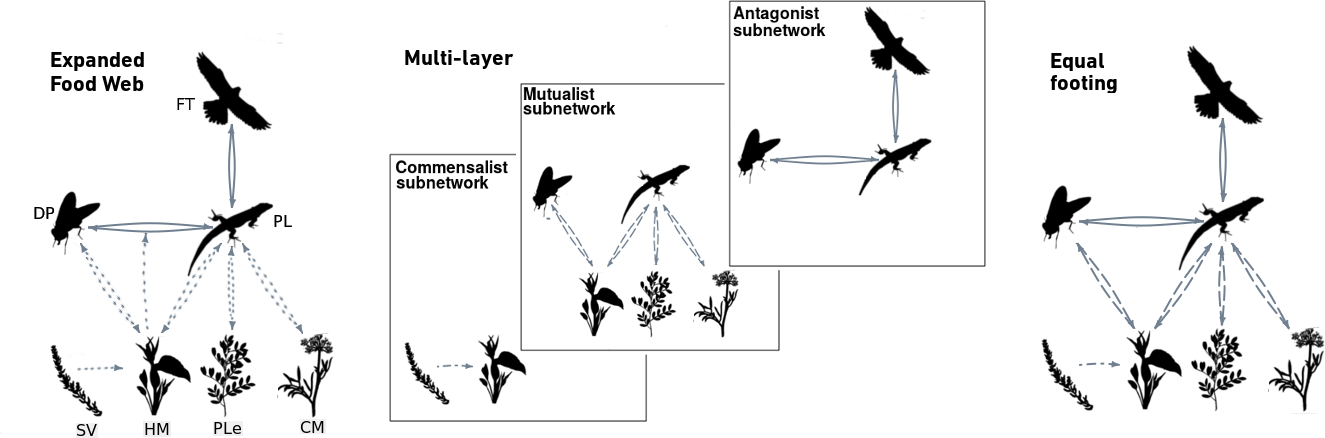
\includegraphics[width=\textwidth]{./Figures/chapter02/Fig_1.png}
\caption[Three approaches for multiple interactions networks]{\color{Gray} Three approaches for constructing and analyzing networks with multiple interaction types. In the first panel, solid lines represent trophic interactions, dotted lines non-trophic ones. Note that frugivory and pollination have both trophic and non-trophic components. In the second and third panels, solid lines represent antagonistic interactions, dashed lines mutualistic ones and dotted-dashed lines commensalistic ones. Data for building the network taken from the Aire Island community (see the Aire Island case study).}
\label{fig:fig2.1}
\end{figure}

\section{Multilayer Networks}
The concept of networks formed by different types of interactions (edges, more generally, connecting two individual nodes of the network) was first developed in the first decades of the 20th century in the field of social sciences, for characterizing social interaction networks with different types of relationships between individuals. Nevertheless, it is only in the last few years that the idea has been properly defined mathematically, given a consistent terminology, and applied to a wide variety of research objectives in, for example, engineering, economical or social networks (see the reviews by \citealt{Boccaletti2014} and \citealt{Kivela2014} to learn more about the history, methodology and applications of the paradigm).

The basic principle is that nodes within a network can be linked in different ways or in different contexts, so that the overall network contains two or more layers that represent different link types or other aspects of variation. Nodes can be connected to nodes of the same layer (intra-layer links) or to nodes of different layers (inter-layer links). Such multidimensional object is called - in it most general definition - a multilayer network. An ecological community in which different species interact in a discrete number of ways is a very intuitive example of such a network \citep{Pilosof2017}. In it, each interaction type would constitute a different layer within the {}'interaction type{}' aspect, and other potential layering aspects could be time (i.e. the realization of the network in different sampling campaigns) or site (different sampling plots).

Mathematically, a multilayer network consists on a quadruplet  $M=\left(V_M,E_M,V,L\right)$  . Its elements are, first, a sequence of sets of elementary layers  $\left\{L_a\right\}_{a=1}^d$  , where  $d$  is the number of layering aspects. The full set of nodes of the network,  $V$  , does not include the information about which node belongs to which layer, so a further set of node-layer tuples encodes this information:  $V_m{\subseteq}V\times L_1\times {\cdots}\times L_d$  . These node-layer tuples, i.e. the instances of a node in a given layer, are called {}'state nodes{}'. Lastly,  $E_m{\subseteq}V_M\times V_M$  is the set of intra-layer and inter-layer links. This minimal definition is expanded in the reviews by \cite{Kivela2014} and \cite{Pilosof2017}. When designing multiple interactions networks,  $d{\geq}1$  , as at least the layering relative to interaction type will be present; also, links may be constrained to {}'diagonal coupling{}', i.e. the situation in which a node will only be connected to itself in different layers. Representations where layers are not interaction types but some other grouping of the community are also possible (Appendix 2.2). For modelling the dynamics of multilayer networks, any dynamical model representing species interactions may be used in which sub-networks are represented by sets of equations and, depending on the design, auxiliary equations may be used to connect the different state nodes of a given entity, or state nodes of different entities in different layers. The inter-layer links of a multilayer network make this framework particularly versatile, as these may represent any kind of relationship between layers (see Appendix A.2.2: Figure A.2.2.3 for a definition of the different types of links in multilayer networks, and their matrix representation). For example, a link coupling the same plant species in pollination and herbivory sub-networks may represent the effect that consumption of reproductive organs by herbivores has in the interactions between the plant and its pollinators. Inter-layer links may also represent a coupling between layers with different temporal or spatial scales, thereby explicitly accounting for the temporal or spatial dimension of the networks. Note that this framework may accommodate networks with markedly different structures. For example, networks where virtually all links are intra-layer and the opposite, networks in which virtually all links are inter-layer, are both multilayer networks; also, networks whose nodes are present in every layer or in just one of them can fall under this framework.

Multilayer networks have been explored in a few studies of multiple interactions networks (Table \ref{tab:table1.1}), but their applicability in ecology goes far beyond these studies. For example, they have been successfully applied to reconstruct super (phylogenetic) trees \citep{vonHaeseler2012}, to study temporal and spatial variability in network structure, or to the analysis of ecological processes at different scales \citep{Pilosof2017} . Despite the potential of the multilayer framework for modelling ecological dynamics within and across layers, most studies listed in Table \ref{tab:table1.1} have only analysed static structural patterns, with the only exceptions being the studies by \cite{Stella2016}, who studied the dynamics of parasite spreading in multilayer ecological networks of varying structures, and by \cite{Gracia-Lazaro2018}, on the influence of inter-layer mutualistic interactions over layers of competitive interactions. In general, ecological studies on multilayer networks are starting to show that interactions other than predator-prey ones are also highly structured \citep{Melian2009,Kefi2015} and this topological structure has important consequences for different community properties \citep{Pocock2012, Evans2013a, Kefi2016a}.

As this approach has been developed mostly in theoretical physics and most reserachers in ecology may not be familiar with its terminology, a brief note is needed here. Following the definitions from \cite{Kivela2014}, a multilayer network is the most general object representing networks with multiple layering aspects and connections among layers. Although we focus on networks where the only layering aspect is interaction type and are diagonally-coupled, (termed `multiplex' networks or `edge-coloured multigraphs' in \citealt{Kivela2014}), we acknowledge that multiple interactions networks can also include other layering aspects and more complex patterns of inter-layer links. Therefore we adopt the more general term of multilayer networks in our review (Box 2). We will also use indistinctly the `layer' and `sub-network' terms to refer to a layer of specific interaction types in this framework.

\section{Equal Footing Networks}

Regardless of the specific characteristics or vital rates of an organism potentially modified by a pairwise interaction, its effects can be summed up as influencing either (1) individual fitness, (2) population size, or (3) population growth rate \citep{Abrams1987}. This view of interactions as aggregating effects over general individual or population-level parameters is the conceptual basis behind {}'equal footing networks{}', with the main consequence that pairwise interactions of any type can be measured and compared {}'on equal footing'.

A minimal population dynamics model can be represented as in Eq. 1. The main difference with the expanded food webs is that here, trophic and non-trophic interactions influence the intrinsic growth rate through the interaction terms of the adjacency matrix  $\left[a_{\mathit{xy}}\right]$  , instead of being modelled through auxiliary equations 2-3. Therefore, the adjacency matrix may include all pairwise combinations \{(0,0),(0,+),(0,-),(+,-),(+,+),(-,-)\} (Appendix A.2.2: Figure A.2.2.4).

Being a more general approach than expanded food webs, numerical models of equal footing networks are more scalable. Following Eq. 1, each species can be modelled by a single equation, and  $S^2+S$ parameters are required for a complete model of  $S$ species. This generality through the integration of fundamentally different interaction mechanisms in the adjacency matrix hinders the level of biological realism that can be achieved, in contrast with expanded food webs. By manipulating the signs of the adjacency matrix, different proportions of interaction types can be generated, but the effect of varying these proportions on community stability is an open question. \cite{Mougi2012} showed that, under certain conditions, local stability is enhanced for theoretical communities mixing antagonism and mutualism, as opposed to communities with a single interaction type. Their a priori conditions were that 1) mutualisms and antagonisms have, in total, the same effect over population growth rates and 2) for any species, the net effect of a given interaction decreases with increasing numbers of links of the same type. Two subsequent studies debated their conclusions: \cite{Suweis2014} stated that these conditions, and not the mixing of interaction types, were the factors that stabilized their models, whereas \cite{Kondoh2015} partially relaxed their initial assumptions and still found increasing stability with interaction mixing. Recently, the methodology developed in \cite{Mougi2012} has been expanded to assess the role of commensalism and amensalism \citep{Mougi2016a} and the potential switching of interactions \citep{Mougi2016b}, finding that separately accounting for these factors (unidirectional interactions and interaction switching) also increases local stability. The evaluation of equal footing networks through local stability analyses (for review see Table \ref{tab:table1.1}) is methodologically equivalent to the analysis of single-interaction networks. Hence, it is a natural approach for comparing networks of single and multiple interaction types without resorting to specific interaction mechanisms. In the studies already published (Table \ref{tab:table1.1}), different studies have considered different sets of interaction types and modelling assumptions, so that no integrative conclusions can be obtained at this point. Nevertheless, an emerging trend seems to be that networks with more than one interaction type and where different interactions are structured non-randomly are more locally stable than their single-interaction, non-structured counterparts.

The equal footing framework can be thought of as a particular type of multilayer network, in which the interaction layers are {}'flattened{}' in a single network, so that inter-layer links disappear, and each node is simultaneously affected by all interactions. \ This flattening is possible when three conditions are met: state nodes of the same node in the different layers of a multilayer network represent the same physical entity (as opposed to transportation networks, for example, where state nodes might represent bus or train stations of the same city), layers are diagonally-coupled, and all interactions in the different layers are expressed in the same units. This last condition is probably the most general, and in fact it represents our second criterion for distinguishing among frameworks. It allows the possibility of flattening multilayer networks in which there is link overlap among layers, as the overall effect will be a function of all layer-specific effects. We believe that these restrictive conditions, and the prevalence of equal footing networks in the theoretical studies listed in Table \ref{tab:table1.1}, merit the consideration of this framework as separated from the more general multilayer networks. The study by \cite{Melian2009} provides an example of a multilayer dataset flattened to an equal footing dynamic model.

\clearpage

\begin{small}
\begin{mdframed}
\subsection*{Box 1: Choosing a multiple interaction network methodology}
%\end{mdframed}
What constitutes a {}'realistic{}' representation of an ecological community? The answer is likely contingent on many factors, including the type of community being studied, the availability of empirical data and/or the ease to obtain it through observational or experimental studies. Although these factors, as well as research objectives and ecological assumptions, vary widely among studies, we propose a series of general guidelines for helping decide which multiple interactions framework is more appropriate for analyzing different types of data and questions (Fig. \ref{fig:fig2.1}).

The first dichotomy is whether the study involves structural and/or dynamical analyses (in this context, dynamical analyses refer to model-based projections of, at least, species abundances or biomass). In the first case, countless studies have analysed network structure based on lists of species and presence/absence of interactions between them. An excellent example of a structural analysis of a multiple interaction network is the comprehensive study of the Chilean rocky shore intertidal community by \cite{Kefi2015}. We suggest, for such analyses, arranging data according to the multilayer framework, which provides a versatile representation of the network and for which there is a well established, wide set of diagnostic metrics \citep{Pilosof2017}.

When values of biomass/abundance and interaction strengths are sampled or estimated (for example, based on allometric relationships, as in e.g. \cite{Kefi2016a}, community dynamics can be modelled. In these cases, the influence of the parameterization on the results obtained should be appropriately gauged against null models, but this topic is out of the scope of our study.

If interactions are classified in terms of their effect over a certain population parameter, either equal footing or multilayer networks are the appropriate modelling frameworks for analyzing dynamical systems. In this situation, choosing one approach over the other depends crucially on our second general criterion, i.e. the units in which interaction strengths are represented. Other factors may also play a role, for example the presence of multilink overlap (see case study), the complexity of inter-layer links, or whether the dynamics of single-interaction sub-networks may be of interest when considered as separate entities. Generalizing, if it is of any interest to consider interaction types separately (for example, if different interaction types are modelled through different functional forms and with different units) or there are complex inter-layer connections, multilayer networks should be used. If, on the other hand, the interest lies in the overall dynamics of the whole system, equal footing networks might be preferable.

The other branch of the flow chart in Fig. \ref{fig:box1.fig1} represents the situation where estimates of interaction strength are classified according to the mechanism they act upon. In this case, if the community consists of relatively few species or functional groups, each interaction can be modelled in detail, and the number of parameters might still be manageable: expanded food webs provide the most appropriate framework for such situations. Modelling the dynamics of a higher number of species, on the other hand, usually implies less mechanistic knowledge of the interactions within the community, and therefore interactions can be grouped in layers of a multilayer network that represent specific families of mechanisms. Notwithstanding these guidelines, as before, other factors may play a role (e.g. the inclusion of interaction modifiers, as in the case study). In all cases, selecting an appropriate framework will ultimately depend on the data at hand, the objectives of the study and the judgement and familiarity of the researchers with the different methodologies.

% within mdframed environments,another float environment does not work well
% so use custom captions of the memoir class
%\begin{figure}[h]
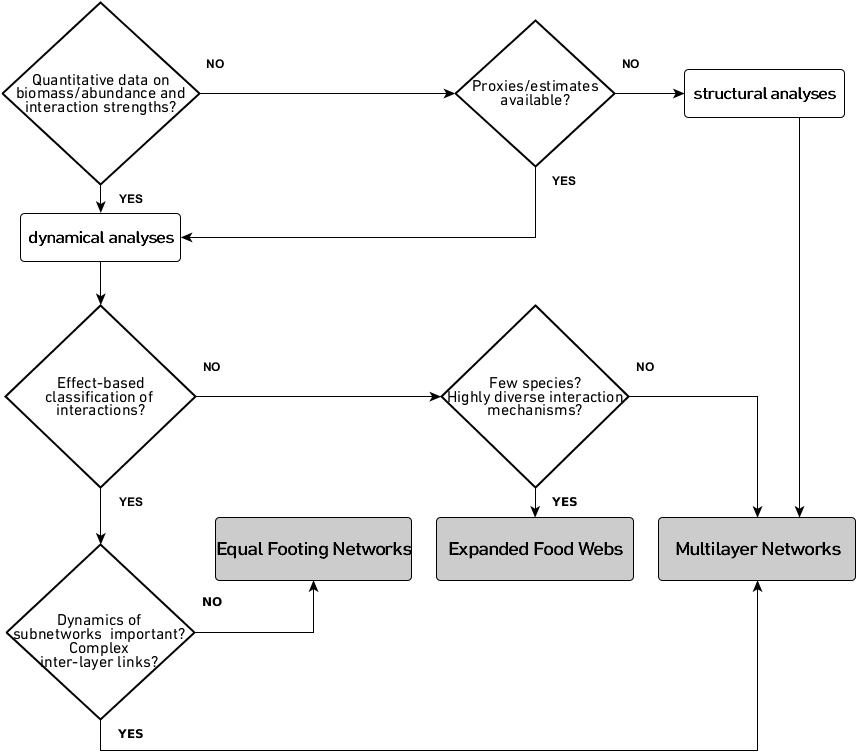
\includegraphics[width=.95\textwidth]{./Figures/chapter02/Box_1_Fig_1.png}
\figcaption[Choosing a multiple interaction network methodology]{\color{Gray} Diagram for choosing a multiple interaction network methodology, to be read starting from the upper left diamond box.}
%\caption}
\label{fig:box1.fig1}
%\end{figure}

\end{mdframed}
\end{small}

\section*{Acquisition and aggregation of empirical data}

Collecting data on the presence and strength of pairwise interactions in nature is notoriously difficult, even for the most easily observed interactions (Jordano 2016). It follows that interaction networks tend to be markedly under{}-sampled \citep{Chacoff2012}, and the proportion of type II errors, i.e. existing interactions that are not observed, is rarely known \citep{Olesen2011a, Morales-Castilla2015, Gravel2016}. In turn, quantifying the strength of observed interactions is also a long-standing challenge even for single interaction networks \citep{Berlow2004}. Several interaction strength indices have been developed by theoretical ecologists, but these are usually disconnected from the set of metrics obtained in field or manipulative studies \citep{Wootton2005}. Furthermore, very few pairwise interaction types have been extensively studied and their functional forms analysed (e.g. \citealt{Holland2002, Novak2008}), while the existence and/or dynamics of the vast majority of interactions in nature remain unknown. Thus, designing and implementing programs for collecting reliable data on multiple interaction types is presently one of the biggest challenges for community ecologists, up to the point that we are aware of just a handful of prominent examples in the literature. For example, \cite{Melian2009} aggregated data from several studies on pollination, seed dispersal and herbivory carried out between 1981-1984 in the Do\~nana Biological Reserve, in southern Spain. With that data, they constructed a network of 390 species and 798 interactions. Parasitic species and links, in addition to predator-prey interactions, were sampled by \cite{Hechinger2011} in food webs of three estuaries in the North American Pacific coast, in a dataset that included 314 species and 11270 interactions. In the study by \cite{Pocock2012}, several interaction types were concurrently sampled in different habitats of an agro{}-ecosystem in the UK, obtaining a network of 560 species and 1501 interactions. Finally, two networks of intertidal communities have been collected recently: \cite{Sander2015} obtained 1898 interactions between 110 taxa from the intertidal middle zone of Tatoosh Island based on observations and natural history of the species, and \cite{Kefi2015} took advantage of decades of work conducted on the marine rocky intertidal communities of the central Chilean coast to reconstruct its qualitative community network based on field observations and expert knowledge. Their network includes 104 species and 4754 interactions.

From these examples, one can distinguish two main strategies for constructing empirical multiple interactions networks: aggregating data from different sources of a given community in order to reconstruct the community network a posteriori (as in \citealt{Melian2009, Hechinger2011, Kefi2015} and \citealt{Sander2015}), or designing an integrated sampling program for a given set of previously defined interaction types, thus obtaining a realization of the network where all interactions are mostly co-occurring in space and time (as in \citealt{Pocock2012}). In the first approach, one may assemble information from studies conducted with different objectives and sampling methodologies and over different time periods, so that the aggregated network can potentially include a large fraction of the realized interactions, but these may or may not co-occur in time and/or space. Differential sampling efforts across studies will be unavoidable, and a posteriori analyses should be considered to minimize over or under-representation of certain clades and interactions. In the second approach, as fieldwork is likely to be conducted in tight time periods and in parallel for the different interaction types, sampling will potentially be more limited. On the other hand, this concurrent sampling is a more realistic snapshot of the co-occurring interactions in the sampling period, and importantly, fieldwork can be designed a priori to assign a near-homogeneous effort to different interaction types (but a posteriori corrections such as sample-based rarefaction are also advised; see \citealt{Pocock2012} and references therein). A non-exhaustive list of factors to account for the design of field campaigns is provided in Table \ref{tab:table1.2}, but a more comprehensive analysis of sampling strategies for multiple interactions networks is needed.

\begin{table} \footnotesize
\caption[Sampling of multiple interaction types]{\color{Gray}List of factors to consider in the design of sampling campaigns for multiple interaction types. These factors are general and independent from the framework chosen to represent the obtained network.}\label{tab:table1.2}
\begin{tabularx}{\textwidth}{p{2cm} X}
\hline
Factor & Examples of relevant questions\\
\hline
Temporal scale &
Single sampling campaign or periodic samples? What is the time scale of the interactions to be sampled? Are all/certain interaction types expected to vary along the sampling period?\\

Spatial scale &
What is the spatial scale of the interactions to be sampled? Are all/certain interaction types expected to vary spatially?\\

Habitat type(s) &
How many habitat types will be sampled? How does sampling effort vary across habitats? Which interaction types are expected to be prevalent in each habitat type?\\

Interaction types &
Which interaction types are expected to be sampled? Which sampling methodologies are applied to capture them? How does the proportion of forbidden links vary among interaction types?\\

Field and experimental observations &
Are experimental observations needed for observing specific interaction types (e.g. for estimating the prevalence of parasitism, or the number of flowers visited by a given pollinator)? How is effort distributed among field and experimental observations?\\

Natural history of species &
Do species in the community have varying activity periods or phenologies? Are there significant differences in mobility, behaviour, and other traits relevant to the probability of observing an interaction?\\

Movement capacity &
Will network include permanent species or also transient ones? How is a permanent species defined?\\
\hline

\end{tabularx}

\end{table}

Regarding the key issue of estimating empirical interaction strengths, it is often necessary to conduct manipulative experiments for obtaining reliable functional forms and interaction strength coefficients. Such experiments, however, are very context and clade-specific, and usually pose increased costs and logistical difficulties over field observations. For these reasons, a growing line of research is being developed for, given minimal information, inferring the presence \citep{Morales-Castilla2015, Deyle2016} and strength \citep{Novak2008, Berlow2009, Vazquez2012} of biotic interactions. Specifically, an interaction strength proxy that may be applicable to different types of interactions is the frequency of occurrence of an interaction. \cite{Poisot2015} proposed a general framework for integrating dynamic interaction strengths in dynamical models, taking into account the long-held idea that the net impact of a species over another can be described as a function of two components: the frequency of interaction and the per interaction effect \citep{Vazquez2005}. Thereby, the relative role of density-mediated and trait-mediated effects on direct interactions can be explicitly analysed. So far, it has been hypothesized that the net impact of mutualistic plant-pollinator interactions can be approximated by their frequency for both sides of the interaction \citep{Vazquez2005,Vazquez2012} and, in addition, that the asymmetry among interaction strengths is well explained in some cases solely by species' relative abundances (for quantitative bipartite networks, as in \citealt{Vazquez2007}). These ideas converge towards a unified neutral view of ecological interactions: interactions can be approximated as being the result of random encounters among individuals, whose probability is mediated by the relative abundances of the populations involved \citep{Araujo2014, Canard2012, Canard2014, Cazelles2016}. The frequency of interactions will naturally equal the net impact of a population over another, since per capita interaction strength will not vary with other factors (traits, environmental conditions). Further research is needed to test the robustness of (1) species abundance as a proxy for interaction frequency, and (2) interaction frequency as a proxy for interaction strength.

\begin{mdframed}
\begin{small}

\subsection*{Box 2: Definitions of key terms}

The approach used for classifying interactions does not only have methodological consequences: it is above all constrained by the very definition of interaction. Hence, it is important to be clear and explicit about the definitions used.

The ones we use in this study for direct and indirect interactions are taken directly from \cite{Abrams1987}. These definitions can be applied both to effect-based and mechanism-based classifications, and though we define indirect interactions for completeness, we mainly focus on direct interactions.

For effect-based classifications, existing definitions are complete, as they cover the full spectrum of possible combinations of interactions in what can be described as the biotic interaction space \citep{Araujo2014}. New terms have been introduced with time, e.g. expanding the definition of (+,-) interactions originally described as being mainly characterized by predation to, first, contramensalism \citep{Arthur1989} and later, antagonism \citep{Sousa1993}.

Within mechanism-based classifications the situation is somewhat more convoluted. In such studies, it is commonplace to study trophic and non-trophic interactions separately. Although defining these terms is apparently trivial, we have encountered very different implicit meanings of what constitutes a non-trophic interaction in the literature. For example, in the studies by \cite{Arditi2005} and \cite{Goudard2008}, non-trophic interactions are defined as modifiers of trophic interactions. \cite{Prasad2010} consider non-trophic interactions to be `driven by one species changing the behaviour but not the density of another species'. Finally, \cite{Kefi2012} interprets non-trophic interactions as being all other interactions than feeding ones, including the non-trophic components of pairwise interactions such as pollination or frugivory. We adopt the latter definition, as it more clearly fits within a simple generalizable framework, although it requires certain interactions to be split in their trophic and non-trophic components. Lastly, effect-based and mechanism-based classifications need not be mutually exclusive \citep{Abrams1987}: it is common for effect-based interaction classes to be divided according to specific ecological mechanisms, e.g. mutualisms can be divided by considering whether there is a trophic component in them or not, etc.

\begin{description}
\item[Interaction] A change in some characteristic of a population mediated by properties or actions by individuals of other population.

\item[Direct interaction] Interaction in which the effect occurs either through direct physical contact or through a third set of entities produced by one of the two interactors.

\item[Indirect interaction] Interaction in which the effect occurs as a result of other effects produced by one interactor on some population property of a third set of entities; and the third set of entities is not produced by any of the interactors.

\item[Trophic interaction] In the context of mechanism-based classifications, an interaction (or component of one) that involves direct exchange of energy (biomass) between the two individuals.

\item[Non-trophic interaction] In the context of mechanism-based classifications, an interaction (or component of one) that does not involve exchange of energy (biomass) between the two interacting individuals.

\item[Single-interaction network] Ecological network in which one interaction type is considered. Classic examples are food webs or plant-pollinator networks.

\item[Multiple interaction network] Ecological network with more than one interaction type. This umbrella term includes any topology and/or classification of interactions.

\item[Expanded food web] Multiple interaction network in which consumer-resource interactions form the basic structure of the network. Other interactions are termed ``non-trophic'' interactions and may affect any parameter of the dynamic model.

\item[Multilayer network] Network with different types of connections between nodes. In an ecological context, different network layers commonly represent different interaction types. If there is only one layering aspect and nodes are diagonally-coupled, that type of multilayer network is termed multiplex.

\item[Equal footing network] Multiple interaction network in which all interaction types are expressed in the same units, i.e. influence the same parameter of the dynamic model.

\end{description}
\end{small}
\end{mdframed}

\section*{The Aire Island case study}

The expanded food web, multilayer and equal footing frameworks for building multiple interactions networks offer complementary insights for the study of ecological communities, and each one is best suited to different types of studies and objectives (Box 1). Here, to demonstrate the diversity of ecological questions that can be addressed with multiple interactions networks, we analyse an empirical community under the lenses of each one of the approaches described. Specifically, we ask:

\begin{enumerate}
\item what is the influence of non-trophic interactions on the local abundances of all species? (expanded food web approach);
\item which species serve as ``hubs'' for linking species through interaction sub-networks and in the overall network? (multilayer network approach);
\item does the strength of different interaction types influences local community stability?(equal footing approach).
\end{enumerate}

The community examined is located on the Aire Island, a small islet located SE off the coast of Menorca (Balearic Islands, Spain) with an area of around 342500 m{\texttwosuperior}. Almost the entire surface of this relatively flat islet is exposed to the effect of the sea. Therefore, most vegetation is halophilous (i.e. thrives in saline environments) except in areas sheltered from wind and sea, where typical Mediterranean species appear, such as Pistacia lentiscus \citep{Perez-Mellado2006}. Our examples are based on a subset of the ecological community of this islet.

A remarkable set of interactions has been unveiled in the Aire Island between the dead horse arum (\textit{Helicodiceros muscivorus}), its associated insect pollinators (Diptera, genus \textit{Calliphora} and \textit{Lucilia}), and the Balearic lizard, \textit{Podarcis lilfordi}. The Balearic lizard is an omnivorous lacertid of medium size, endemic to the Balearic Islands. It has been shown to bask on the spathe of \textit{Helicodiceros muscivorus} {}' flowers, and to feed on the pollinating flies attracted by the intense odour produced by the plant. In addition to this negative effect of \textit{Podarcis lilfordi} on \textit{Helicodiceros muscivorus} through consumption of potential pollinators, it is itself an effective seed disperser of the plant: \textit{Podarcis lilfordi} consumes ripe fruits of \textit{Helicodiceros muscivorus} routinely, and seeds dispersed by the lizard show a significantly higher probability of germination than non-consumed seeds \citep{Perez-Mellado2006}. \textit{Podarcis lilfordi} is also an effective pollinator of other species at Aire Island. Particularly, high loads of pollen from \textit{Pistacia lentiscus} and \textit{Crithmum maritimum} have been found in lizard's bodies in previous studies on the same community \citep{Perez-Mellado2000}. Due to the scarcity of natural predators, \textit{Podarcis lilfordi} reaches high densities in the islet \citep{Perez-Mellado2008}. Its main predator is probably the Eurasian Kestrel (\textit{Falco tinnunculus}), that does not nest on the islet but visits it frequently. Lastly, the appearance of \textit{Helicodiceros muscivorus} is related to the percentage of soil covered by \textit{Suaeda Vera}, an hallophylous shrub of the Chenopodiaceae family, suggesting facilitation by the shrub on the development of \textit{Helicodiceros muscivorus} \citep{Perez-Mellado2006}. The interaction network formed by these 7 species (or guild, in the case of the Diptera) spans 3 trophic levels, and includes antagonistic, mutualistic and commensalistic interactions. In the following equations and figures, $S$ refers to the whole set of species, and species are denoted by their initials or silhouettes. When available, we use empirical data for parameter estimates. Whenever empirically derived estimates are unavailable, as these examples are only to illustrate the approaches, we assign values based on our judgements of plausibility.

\subsection*{Expanded food webs: Influence of non-trophic interactions in equilibrium abundances}

The main strength of the expanded food webs is the inclusion of detailed, mechanistic, non-trophic interactions in the general food web structure. We investigated their influence in the resulting abundance patterns of the community, compared to a standard food web model.

The continuous-time model for the expanded food web considers only three ecological processes: growth, mortality, and pairwise interactions, which can be trophic or non-trophic. Trophic interactions can, themselves, be modified by the presence of a third species. The main equations are of the form:

\begin{equation} \label{eq:2.4}
\frac{\mathit{dN}_x}{\mathit{dt}}=r_xN_x-m_xN_x^2+\sum _{y{\in}S,y{\neq}x}a_{\mathit{xy}}N_xN_y
\end{equation}

where  $r_x$  is the short-term per capita growth rate,  $m_x$ is the per capita mortality rate (that, multiplied by  $N_x^2$  , acts as a self-limitation term) and  $a_{\mathit{xy}}$  are the pairwise trophic interaction coefficients (the partial derivative of the per capita growth rate of species  $x$  with respect to the density of species  $y$  ).

Several non-trophic interactions are included on top of this general structure, affecting either  $r_x$ ,  $m_x$ or  $a_{\mathit{xy}}$ . As an example, the modification of the mortality rate is modelled with a saturating function \citep{Kefi2012}

\begin{equation} \label{eq:2.5}
m_x\left(N_y\right)=\frac{m_x^{\mathit{NTI}}N_y+m_x^0N_y^0}{N_y+N_y^0}
\end{equation}

The function varies between a basal value $m_x^0$ when $N_y=0$ , i.e. in the absence of non-trophic interactions, and  $m_x^{\mathit{NTI}}$ when the non-trophic interaction is highest. The same equation was used to model non-trophic interactions influencing the other parameters of Eq. 6 (growth rates  $r_x$ and interaction coefficients  $a_{\mathit{xy}}$ ). For modelling the Aire Island community, we assumed that (1) all mutualistic interactions positively affect short-term growth rates, i.e. $r_x^{\mathit{NTI}}>r_x^0$ for \textit{Helicodiceros muscivorus}, \textit{Podarcis lilfordi}, Diptera, \textit{Pistacia lentiscus} and \textit{Crithmum maritimum}; (2) the presence of \textit{Suaeda vera} increases the survival probability of \textit{Helicodiceros muscivorus} seedlings by providing a favorable microhabitat, thus decreasing the mortality rate of the facilitated plant, i.e. $m_{\mathit{HM}}^{\mathit{NTI}}<m_{\mathit{HM}}^0$ ; and (3) increases in abundance of \textit{Helicodiceros muscivorus} increased the magnitude of the predator-prey interaction between \textit{Podarcis lilfordi} and the Diptera species, i.e. $a_{\mathit{PL},\mathit{DP}}^{\mathit{NTI}}>a_{\mathit{PL},\mathit{DP}}^0$ and $a_{\mathit{DP},\mathit{PL}}^{\mathit{NTI}}<a_{\mathit{DP},\mathit{PL}}^0$.

The complete parameterizations of the expanded food web model and the equal footing model are included in Appendix 2.1. We found significant differences in abundances at equilibrium for all species except \textit{Suaeda vera}, depending on the set of interactions considered (Fig. \ref{fig:fig2.2}). We define equilibrium as the steady state reached after a sufficient number of time steps (2500 in our case). Non-trophic interactions in the Aire Island community are all positive, and accordingly, all populations increase in equilibrium abundance when engaging in non-trophic interactions. The only organism that conceivably could be negatively affected by the inclusion of non-trophic interactions are the Diptera, given that the magnitude of the \textit{Podarcis lilfordi} - Diptera antagonism is enhanced by higher abundance of \textit{Helicodiceros muscivorus}. With the parameterization chosen, however, the positive influence of the Diptera -- \textit{Helicodiceros muscivorus} mutualism outweighs this increase (Fig. \ref{fig:fig2.2}, note the increase in Diptera abundance when non-trophic interactions are considered). Note that this is the only approach in which we explicitly model the influence of \textit{Helicodiceros muscivorus} populations in the predator-prey interaction between the Diptera species and \textit{Podarcis lilfordi}.

\begin{figure}[ht]
\centering
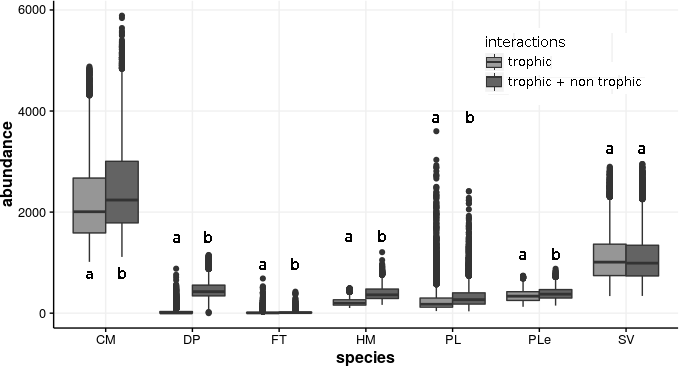
\includegraphics[width=\textwidth]{./Figures/chapter02/Fig_2.png}
\caption[Expanded Food Web analysis]{\color{Gray} Equilibrium abundances of the Aire Island community when considering trophic interactions, or trophic and non-trophic ones. Boxplots with different letters are significantly different according to Wilcoxon rank-sum tests (CM: W = 38176000, p {\textless} 0.05; DP: W = 63730000, p {\textless} 0.05; FT: W = 38512000, p {\textless} 0.05; HM: W = 57170000, p {\textless} 0.05; PL: W = 42005000, p {\textless} 0.05; PLe: W = 38454000, p {\textless} 0.05; SV: W = 31595000, p = 0.059).}
\label{fig:fig2.2}
\end{figure}

\subsection*{Multilayer networks: Importance of each species in structuring the network}

The role of the different species in structuring a given community has been extensively assessed for single-interaction networks \citep{Coux2016} and for multilayer networks in other fields \citep{Sole-ribalta2014,DeDomenico2015a}. For the multilayer framework, several metrics have been adapted directly from single-interaction networks and others have been defined taking into account the multidimensional nature of the multilayer approach \citep{DeDomenico2015a}. Among these novel metrics, the concept of multidegree is a multidimensional extension of the degree of a single-interaction network, that may help uncover important, well-connected species in each sub-network and in the overall structure. Here we calculate multidegrees as defined in \cite{Boccaletti2014}, where formal definitions are provided.

For understanding the concept of multidegrees, we first need to define the multilinks of the network. Multilinks (or multiedges) are links connecting two nodes in a combination of layers. For example, the Aire Island network has three interaction types. A multilink of the form (1,0,0) exists between two species if these species are connected in the first layer and not in the second or third one. One can see thus that the number of potential multilinks between any two species in a general network with  $M$  layers is  $2^M$  . The multidegrees  $m_x^i$ of species  $i$ are its number of multilinks of type  $x$, and its aggregation,  $m^i$  , is the overall multidegree as considered e.g. in \cite{Stella2016}.

Given three layers representing interaction types \{antagonism, commensalism, mutualism\}, the multilinks for the Aire Island network are:

\begin{equation*}
\begin{matrix}m_0=\{0,0,0\}\\m_1=\{0,0,1\}\\m_2=\{0,1,0\}\\m_3=\{0,1,1\}\\m_4=\{1,0,0\}\\m_5=\{1,0,1\}\\m_6=\{1,1,0\}\\m_7=\{1,1,1\}\end{matrix}
\end{equation*}

where  $m_0$ is the null multilink, representing the situation in which two species are not connected in any layer, and subsequently,  $m_7$ represents a multilink whereby two species are connected in the three layers. The number of shared multilinks between any two species can be represented by multi-adjacency matrices. The multi-adjacency matrices of the Aire Island community are:

\begin{equation*}
A^{m_0}=\begin{matrix}\text{ }\\\left.\phantom{\begin{matrix}\mathit{FT}\\\mathit{PL}\\\mathit{DP}\\\mathit{HM}\\\mathit{SV}\\\mathit{PLe}\\\mathit{CM}\end{matrix}}\right(\end{matrix}\begin{matrix}\mathit{FT}&\mathit{PL}&\mathit{DP}&\mathit{HM}&\mathit{SV}&\mathit{PLe}&\mathit{CM}\\0&0&1&1&1&1&1\\0&0&0&0&1&0&0\\1&0&0&0&1&1&1\\1&0&0&0&0&1&1\\1&1&1&0&0&1&1\\1&0&1&1&1&0&1\\1&0&1&1&1&1&0\end{matrix}\begin{matrix}\text{ }\\\left)\phantom{\begin{matrix}\mathit{FT}\\\mathit{PL}\\\mathit{DP}\\\mathit{HM}\\\mathit{SV}\\\mathit{PLe}\\\mathit{CM}\end{matrix}}\right.\end{matrix}\begin{matrix}\text{ }\\\mathit{FT}\\\mathit{PL}\\\mathit{DP}\\\mathit{HM}\\\mathit{SV}\\\mathit{PLe}\\\mathit{CM}\end{matrix}
\end{equation*}

\bigskip

\begin{equation*}
A^{m_1}=\begin{matrix}\text{ }\\\left.\phantom{\begin{matrix}\mathit{FT}\\\mathit{PL}\\\mathit{DP}\\\mathit{HM}\\\mathit{SV}\\\mathit{PLe}\\\mathit{CM}\end{matrix}}\right(\end{matrix}\begin{matrix}\mathit{FT}&\mathit{PL}&\mathit{DP}&\mathit{HM}&\mathit{SV}&\mathit{PLe}&\mathit{CM}\\0&0&0&0&0&0&0\\0&0&0&1&0&1&1\\0&0&0&1&0&0&0\\0&1&1&0&0&0&0\\0&0&0&0&0&0&0\\0&1&0&0&0&0&0\\0&1&0&0&0&0&0\end{matrix}\begin{matrix}\text{ }\\\left)\phantom{\begin{matrix}\mathit{FT}\\\mathit{PL}\\\mathit{DP}\\\mathit{HM}\\\mathit{SV}\\\mathit{PLe}\\\mathit{CM}\end{matrix}}\right.\end{matrix}\begin{matrix}\text{ }\\\mathit{FT}\\\mathit{PL}\\\mathit{DP}\\\mathit{HM}\\\mathit{SV}\\\mathit{PLe}\\\mathit{CM}\end{matrix}
\end{equation*}

\bigskip

\begin{equation*}
A^{m_2}=\begin{matrix}\text{ }\\\left.\phantom{\begin{matrix}\mathit{FT}\\\mathit{PL}\\\mathit{DP}\\\mathit{HM}\\\mathit{SV}\\\mathit{PLe}\\\mathit{CM}\end{matrix}}\right(\end{matrix}\begin{matrix}\mathit{FT}&\mathit{PL}&\mathit{DP}&\mathit{HM}&\mathit{SV}&\mathit{PLe}&\mathit{CM}\\0&0&0&0&0&0&0\\0&0&0&0&0&0&0\\0&0&0&0&0&0&0\\0&0&0&0&1&0&0\\0&0&0&1&0&0&0\\0&0&0&0&0&0&0\\0&0&0&0&0&0&0\end{matrix}\begin{matrix}\text{ }\\\left)\phantom{\begin{matrix}\mathit{FT}\\\mathit{PL}\\\mathit{DP}\\\mathit{HM}\\\mathit{SV}\\\mathit{PLe}\\\mathit{CM}\end{matrix}}\right.\end{matrix}\begin{matrix}\text{ }\\\mathit{FT}\\\mathit{PL}\\\mathit{DP}\\\mathit{HM}\\\mathit{SV}\\\mathit{PLe}\\\mathit{CM}\end{matrix}
\end{equation*}

\bigskip

\begin{equation*}
A^{m_4}=\begin{matrix}\text{ }\\\left.\phantom{\begin{matrix}\mathit{FT}\\\mathit{PL}\\\mathit{DP}\\\mathit{HM}\\\mathit{SV}\\\mathit{PLe}\\\mathit{CM}\end{matrix}}\right(\end{matrix}\begin{matrix}\mathit{FT}&\mathit{PL}&\mathit{DP}&\mathit{HM}&\mathit{SV}&\mathit{PLe}&\mathit{CM}\\0&1&0&0&0&0&0\\1&0&1&0&0&0&0\\0&1&0&0&0&0&0\\0&0&0&0&0&0&0\\0&0&0&0&0&0&0\\0&0&0&0&0&0&0\\0&0&0&0&0&0&0\end{matrix}\begin{matrix}\text{ }\\\left)\phantom{\begin{matrix}\mathit{FT}\\\mathit{PL}\\\mathit{DP}\\\mathit{HM}\\\mathit{SV}\\\mathit{PLe}\\\mathit{CM}\end{matrix}}\right.\end{matrix}\begin{matrix}\text{ }\\\mathit{FT}\\\mathit{PL}\\\mathit{DP}\\\mathit{HM}\\\mathit{SV}\\\mathit{PLe}\\\mathit{CM}\end{matrix}
\end{equation*}

\bigskip

\begin{equation*}
A^{m_3}=A^{m_5}=A^{m_6}=A^{m_7}=0
\end{equation*}

The multidegrees of the seven species of the community are the number of multilinks incident to them (Table \ref{tab:table1.3}). These metrics show that \textit{Podarcis lilfordi} is the most connected species, overall and both in the mutualist and antagonist sub-networks. \textit{Helicodiceros muscivorus} and Diptera are the following species in multidegree, and their links also span two layers. All other species are represented only in one layer, and are only connected to \textit{Podarcis lilfordi}, inviting the interpretation that the Balearic lizard has a disproportionate importance in structuring the community. In our small community, these results are visually evident, but the multidegree concept can be very useful in highly populated networks, where the importance of different species across layers is not obvious from visual inspection of the data. Note that by decomposing the overall multidegree into the contributions of each multilink we are able to evaluate the potential link overlap of any pair of species in any combination of layers. In our simple example, however, there is no overlap, a reasonable assumption when considering an effect-based classification of interactions over a single population parameter, since the potential partial positive and negative effects of a species over another are aggregated in order to calculate the net effect and the associated interaction type. For example, looking again at the \textit{Podarcis} -- \textit{Helicodiceros} interaction, the net direct effect of the lizard over the plant could be decomposed in, at least, 1) a negative effect due to the consumption of fruits (i.e. the trophic part of the pairwise interaction), 2) another negative effect due to the predation of potential Diptera pollinators, 3) the positive effect on seed dispersal, and 4) a further positive effect on survival of seeds that have been dispersed by \textit{Podarcis lilfordi} as opposed to seeds that germinate naturally. In the absence of more detailed experiments, and as suggested by \cite{Perez-Mellado2006}, we considered the overall effect of \textit{Podarcis lilfordi} over \textit{Helicodiceros muscivorus} to be positive. Link overlap in interactions can be expected when two species interact in different ways, for example due to varying ecologies of life stages, and more generally when the temporal dimension is included in the analyses.

\begin{table} \small
\caption[Multidegrees of the Aire Island multilayer network]{\color{Gray}Multidegrees of the seven species of the Aire Island multilayer network. Note that the trivial $m_0$ multilink represents no connections, so it is not considered for calculating the overall multidegree $m$.}\label{tab:table1.3}
\begin{tabularx}{\textwidth}{p{4cm}XXXXXXXXX}
\hline
& $m_0$ & $m_1$ & $m_2$ & $m_3$ & $m_4$ & $m_5$ & $m_6$ & $m_7$ & $m$\\ \hline
Falco tinnunculus & 5 & 0 & 0 & 0 & 1 & 0 & 0 & 0 & 1\\
Podarcis lilfordi & 1 & 3 & 0 & 0 & 2 & 0 & 0 & 0 & 5\\
Diptera & 4 & 1 & 0 & 0 & 1 & 0 & 0 & 0 & 2\\
Helicodiceros \ muscivorus & 3 & 2 & 1 & 0 & 0 & 0 & 0 & 0 & 3\\
Suaeda vera & 5 & 0 & 1 & 0 & 0 & 0 & 0 & 0 & 1\\
Pistacia lentiscus & 5 & 1 & 0 & 0 & 0 & 0 & 0 & 0 & 1\\
Crithmum maritimum & 5 & 1 & 0 & 0 & 0 & 0 & 0 & 0 & 1\\ \hline
\end{tabularx}

\end{table}


\subsection*{Equal footing networks: Influence of the magnitude of mutualistic and antagonistic interactions on community stability}

For assessing the effect of the strength of different interaction types on the overall stability of the network, we modelled the community using the equal footing framework. We used the continuous-time logistic equations proposed by \cite{Garcia-Algarra2014}, in which all extrinsic effects -- environmental, biotic interactions -- fall on the intrinsic growth rate  $r_x$ :

\begin{equation} \label{eq:6}
\frac{\mathit{dN}_x}{\mathit{dt}}=r_xN_x
\end{equation}

where

\begin{equation} \label{eq:7}
r_x=r_x^0+\sum _{y{\in}S,y{\neq}x}a_{\mathit{xy}}N_y-\left(\beta _x+c_x\sum _{y{\in}S,y{\neq}x}a_{\mathit{xy}}N_y\right)N_x
\end{equation}

The rightmost term of Eq.9 represents the self-limitation term. In the absence of pairwise interactions, the parameter $\beta _x$ controls self-limitation, and $c_x$ is a proportionality constant. Pairwise interaction coefficients  $a_{\mathit{xy}}$ were assumed constant. For assessing the relative influence of different interaction types on community stability, we varied the relative magnitude of facilitative (commensalistic and mutualistic interactions) and antagonistic coefficients and analysed the resulting local stability patterns of the system by examining the sign of the leading eigenvalue of the associated Jacobian matrix (Fig. \ref{fig:fig2.3} and Appendix A.2.3: Figure A.2.3.2).

Parameterizations with weak antagonistic interactions were virtually all stable (19991 out of 20000 replicates), regardless of the magnitude of facilitative interaction strength (Fig. \ref{fig:fig2.3}, groups a and b). Communities parameterized with strong antagonistic interactions (group c in Fig. \ref{fig:fig2.3}), on the other hand, were mostly unstable, with only 20 out of 10000 replicates having a leading eigenvalue {\textless} 0. All unstable communities were also unfeasible in that either key species went extinct or some species grew unbounded despite the self-limitation term of Eq. 9. Interaction strength magnitudes were chosen arbitrarily, in the absence of empirical data, but patterns were robust to variations of +- 2 orders of magnitude. Our results therefore suggest that increasing antagonist interaction strengths for this particular community would lead to instability. Bear in mind, though, that local stability analyses are only an approximation of ecological stability, as they only apply to closed systems in equilibrium. If accepting this assumption, local instability in the Aire Island community could be interpreted as being triggered by increased per capita antagonistic interaction strengths. These could appear, for example, if sexual dimorphism in \textit{Podarcis lilfordi} led to higher predation of females by birds, thus exerting a higher influence on population growth rate. This, however, does not seem to be case, since the only dimorphism reported in Aire Island is the slightly larger body size of males \citep{Perez-Mellado2000}; hence, no differential predation is expected.


\begin{figure}[!ht]
\centering
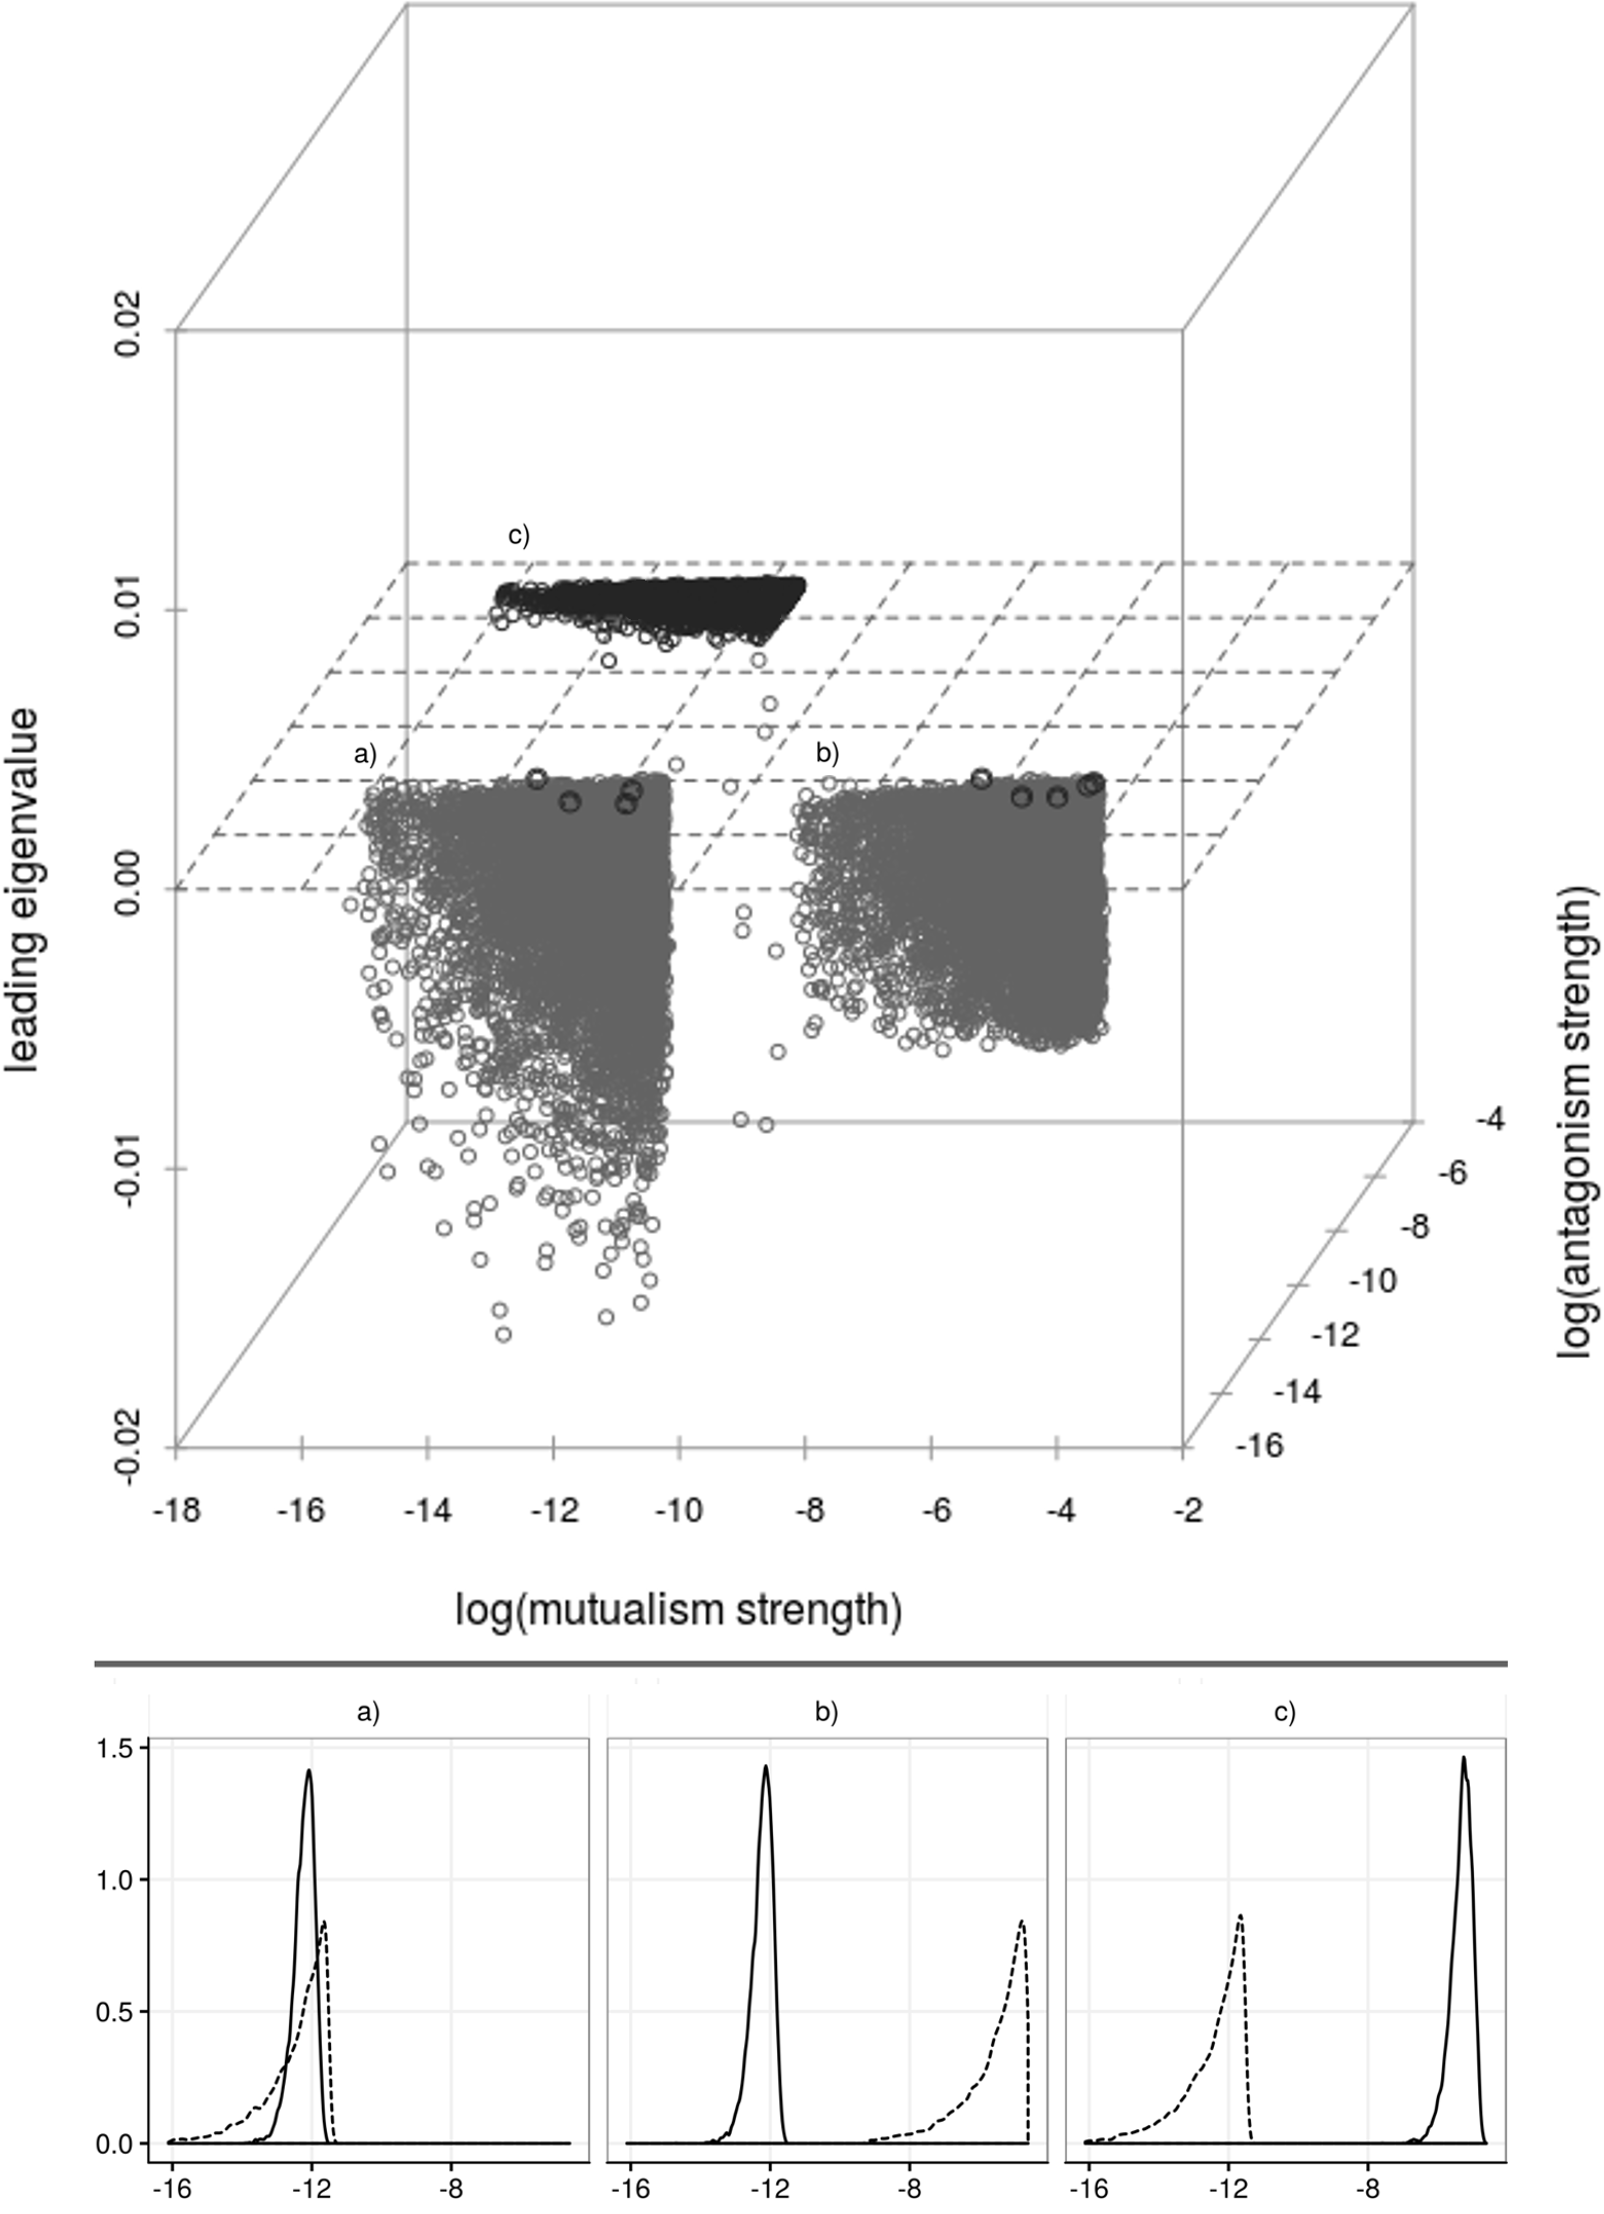
\includegraphics[width=.75\textwidth]{./Figures/chapter02/Fig_3.png}
\caption[Equal footing network analysis]{\color{Gray} Distribution of antagonistic and mutualistic interaction strengths and the leading eigenvalue of the resulting system. In the scatterplot, grey circles are systems with leading eigenvalue < 0, and black circles are systems with leading eigenvalue > 0. Group a) is the group of simulations with weak antagonistic and facilitative interactions; group b) are simulations with weak antagonistic and strong facilitative interactions; group c) are simulations with strong antagonistic and weak facilitative interactions. Within group c) only eigenvalue magnitudes close to 0 are shown, due to the extreme variability of the raw data (with values up to $10^99$ ). The rest of the data is shown in Appendix A.2.3: Figure A.2.3.2. For reference, a grid is drawn representing the z = 0 plane. Lower panels show the density distribution, for each group, of the logarithm of antagonist interaction strengths (solid lines) and the logarithm of facilitative interaction strengths (dashed lines).}
\label{fig:fig2.3}
\end{figure}


\section{Lessons from the case study}

In the Aire Island, the ecological community studied is structured around \textit{Podarcis lilfordi}, due to its high density and its key role as omnivorous feeder as well as seed disperser and pollinator of several plant species. This species and \textit{Helicodiceros muscivorus} are the ones most connected in the network, as shown by the multidegree analysis. Non-trophic interactions are key for correctly projecting population abundances, supporting empirical observations of the importance of facilitation between plant species \citep{Perez-Mellado2006} and effective seed dispersal by \textit{Podarcis lilfordi} \citep{Perez-Mellado2000}. We posit that the role of non-trophic interactions, as modelled in the expanded food web approach, will vary among communities and studies, but it is essential to integrate them in food web analyses, particularly for fine-scale and well-studied systems. Lastly, with the equal footing approach, we have shown that if we assume all interactions to influence intrinsic growth rates, the strength of antagonistic interactions controls the local stability of the network by potentially driving \textit{Podarcis lilfordi} or the Diptera pollinators to extinction. Specifically, even if no local extinctions occur, the variability on the \textit{Podarcis} abundances driven by an increase in antagonistic interaction strengths can destabilize the community, due to its central position on the network (as shown by the multidegree analysis). Positive interactions, in turn, can vary in magnitude without significant effects on local stability.

The results shown here, however, are merely to exemplify the application of the three methodologies on different ecological questions. Different methodologies evaluating the same problem may yield varying results; for example, equilibrium abundances of stable simulations obtained with the equal footing approach (Appendix A.2.3: Figure A.2.3.1) vary significantly from those obtained with the expanded food webs (Fig. \ref{fig:fig2.2}). Choosing an appropriate formulation is not an exact science, as it involves a balance between available spatiotemporal data on species and interactions, natural history knowledge of the system, parsimony of the mathematical model, and objectives of the study (Box 1). In this particular community, in which the number of species is limited and the main interactions and mechanisms are relatively well-known, we advocate for more in-depth analyses based on expanded food webs, that may be parameterized with the results of manipulative studies of, e.g. localised removal of certain species or seed dispersal experiments for obtaining estimates of interaction strength.

\section{Network ecology moving forward}

Communities are comprised of individuals of different species interacting dynamically, and the wide variety of interactions any species engages in is key to its survival and thriving. Incorporating the effects of multiple interaction types in network analyses provides a more complete picture of community dynamics than relying on networks of a single interaction type. We have shown that frameworks for the study of multiple interactions networks are sufficiently mature and can accommodate a wide variety of research objectives and types of empirical data. We hope that the improved understanding of these frameworks, and the explicit recognition of their relative limitations and advantages, will lead to designing field studies that adequately capture the variety of interactions in communities, thus going beyond traditional approaches focusing on single interactions and often single clades. Questions in community ecology that remain unanswered can be addressed with a multiple interactions networks approach to the analysis of ecological communities. For example, we have little knowledge regarding the proportion among different types of interactions in real communities, whether this proportion is constant, whether it varies with any intrinsic or extrinsic factor, or whether it is related to community stability. Furthermore, it is unclear whether the trophic position of a species is related to the type of interactions it is more likely to be engaged in. Likewise, we have little knowledge of whether a species deemed important in a given sub-network will generally have such a role in sub-networks of other interaction types. Because observation of interaction strength in natural systems is extremely difficult to document, integration of empirical data and modelling frameworks requires that consistent interaction strength proxies be designed and tested. The neutral interactions hypothesis is a promising starting point for providing a metric applicable to all interaction types, but it needs to be tested for different communities and interaction types. On the other hand, the application of expanded food webs models to specific communities can trigger the design of manipulative studies to assess the functional forms and dynamics of non-trophic interactions, most of which remain unknown despite their importance.

These and other related questions are fundamental in order to understand the response of ecological communities to perturbations such as climate change or habitat loss. In summary, the development of theoretical models, such as the ones presented here, needs to be contrasted with multipe field or experimental studies for different community types.
